\documentclass[12pt]{article}
\usepackage[utf8]{inputenc}

\usepackage{enumitem}
\usepackage[margin=2cm]{geometry}

\usepackage{amsmath, amsfonts, amssymb}
\usepackage{graphicx}
\usepackage{tikz}
\usepackage{pgfplots}
\usepackage{multicol}

\usepackage{comment}
\usepackage{url}
\usepackage{calc}
\usepackage{subcaption}
\usepackage{circledsteps}

\usepackage{array}

\setlength\parindent{0pt}

\usepackage{fancyhdr}
\pagestyle{fancy}
\fancyhf{}
\renewcommand{\headrulewidth}{2pt}
\renewcommand{\footrulewidth}{0pt}
\rfoot{\thepage}
\lhead{\textsc{Math} 244}
\chead{\textsc{Homework 6}}
\rhead{Fall 2023}

\pgfplotsset{compat=1.16}

% MATH commands
\newcommand{\ga}{\left\langle}
\newcommand{\da}{\right\rangle}
\newcommand{\oa}{\left\lbrace}
\newcommand{\fa}{\right\rbrace}
\newcommand{\oc}{\left[}
\newcommand{\fc}{\right]}
\newcommand{\op}{\left(}
\newcommand{\fp}{\right)}

\newcommand{\bi}{\mathbf{i}}
\newcommand{\bj}{\mathbf{j}}
\newcommand{\bk}{\mathbf{k}}
\newcommand{\bF}{\mathbf{F}}

\newcommand{\ra}{\rightarrow}
\newcommand{\Ra}{\Rightarrow}

\newcommand{\sech}{\mathrm{sech}\,}
\newcommand{\csch}{\mathrm{csch}\,}
\newcommand{\curl}{\mathrm{curl}\,}
\newcommand{\dive}{\mathrm{div}\,}

\newcommand{\ve}{\varepsilon}
\newcommand{\spc}{\vspace*{0.5cm}}

\DeclareMathOperator{\Ran}{Ran}
\DeclareMathOperator{\Dom}{Dom}

\newcommand{\exo}[3]{\noindent\textcolor{red}{\fbox{\textbf{Section {#1}, Problem {#2}}}\hrulefill   \textbf{({#3} Pts})}\vspace*{10pt}}

\begin{document}
\thispagestyle{empty}
	\noindent \hrulefill \newline
	MATH-244 \hfill Pierre-Olivier Paris{\'e}\newline
	Homework 6 Solutions \hfill Fall 2023\newline \vspace*{-0.7cm}
	
	\noindent\hrulefill
	
	\spc

	\exo{15.8}{2}{5}

	\begin{enumerate}[label=(\alph*)]
		\item We have $$x = \rho \cos \theta \sin \phi = 2 \cos (\pi / 2 ) \sin (\pi /2 ) = 0,$$ $$y = \rho \sin \theta \sin \phi = 2 \sin (\pi /2) \sin (\pi /2 ) = 2,$$ and $$z = \rho \cos (\phi ) = 2 \cos (\pi /2 ) = 0$$. 
		\item We have $$x = 4 \cos (-\pi /4) \sin (\pi / 3) = 4 (\sqrt{2}/2) (\sqrt{3}/{2}) = \sqrt{6},$$ $$y = 4 \sin (-\pi/4) \sin (\pi / 3) = 4 (-\sqrt{2}{2})(\sqrt{3}/2) = -\sqrt{6}$$ and $$z = \rho \cos (\pi /3 ) = 4 (1/2) = 2.$$
	\end{enumerate}

	\exo{15.8}{12}{5}

	There is no restriction on the angle $\theta$. Writing $\rho = \sqrt{x^2 + y^2 + z^2}$, we see that $1 \leq \sqrt{x^2 + y^2 + z^2} \leq 2$. Therefore, the solid lies between two spheres centered at the origin of radius $1$ and $2$ respectively. The latitude $\phi$ is between $\pi/2$ and $\pi$. Here is an illustration of the solid:
	\begin{center}
	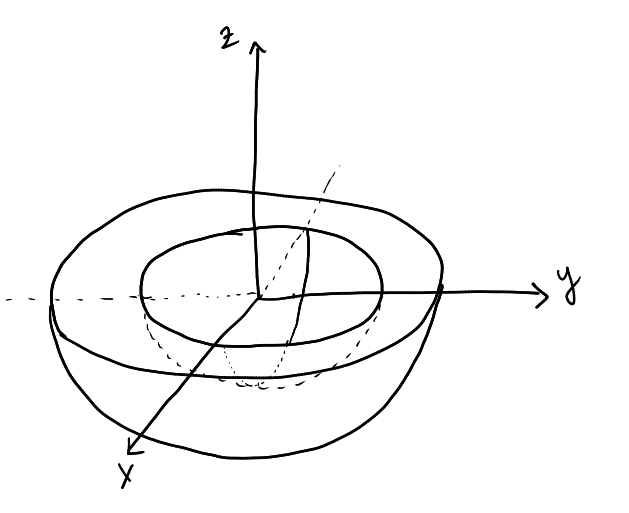
\includegraphics[scale=0.35]{prob12-15-8.png}
	\end{center}
	It looks like half of the Earth with the center removed (the inner core). 

	\newpage

	\exo{15.8}{22}{10}

	In spherical coordinates, we have
	\begin{equation}
		E = \{ (\rho , \theta , \phi ) \, : \, 0 \leq \rho \leq 1 , \, 0 \leq \theta \leq 2 \pi , \, 0 \leq \phi \leq \pi / 3 \} .
	\end{equation}
	Changing to spherical coordinates, we get
	\begin{align*}
	\iiint_E y^2 z^2 \, dV &= \int_0^{\pi/3} \int_0^{2\pi} \int_0^1 (\rho^2 \sin^2 (\theta ) \sin^2 (\phi ))(\rho^2 \cos^2 (\phi)) \rho^2 \sin \phi \, d\rho d \theta d\phi \\ 
	&= \int_0^{\pi/3} \int_0^{2\pi} \int_0^1 \rho^6 \sin^2 (\theta ) \sin^3 (\phi) \cos^2 (\phi ) \, d\rho d \phi d \theta \\ 
	&= \Big( \int_0^1 \rho^6 \, d\rho \Big) \Big( \int_0^{2\pi} \sin^2 (\theta ) \, d\theta \Big) \Big( \int_0^{\pi/3} \sin^2 (\phi ) \cos^2 (\phi ) \sin (\phi ) \, d\phi \Big) \\ 
	&=  \\
	&= \int_0^{\pi/3} \int_0^{2\pi} \int_0^1 \rho^5 \sin^2 (\theta ) \cos^2 (\phi ) \, d \rho d \theta d \phi \\ 
	&= \Big( \frac{1}{7} \Big) \Big( \Big) \Big( \int_0^{\pi/3} (1 - \cos^2 (\phi ) ) \cos^2 (\phi) \sin (\phi ) \, d \phi \Big)
	\end{align*}
Letting $u = \cos \phi$, we get $du = - \sin (\phi ) \, d\phi$ and therefore
	\begin{align*}
	\int_0^{\pi/3} (1 - \cos^2 (\phi )) \cos^2 (\phi) \sin (\phi) \, d\phi &= \int_1^{1/2} (1 - u^2) u^2 (-du) \\
	&= \int_{1/2}^1 u^2 - u^4 \, du \\ 
	&= \frac{47}{480} .
	\end{align*}
Hence, denoting the original integral by $I$, 
	\begin{align*}
	I &=\Big( \frac{1}{7} \Big) \Big( \pi \Big) \Big( \frac{47}{480} \Big) \approx 0.0439. \tag*{$\triangle$}
	\end{align*}


	\exo{15.8}{26}{10}

	In spherical coordinates, the cone $z = \sqrt{x^2 + y^2}$ is $\phi = \pi/4$. The equations of the two spheres becomes $\rho = 1$ and $\rho = 2$. Therefore, the solid $E$ can be described as followed:
	\begin{equation}
		E = \{ (\rho , \theta , \phi ) \, : \, 1 \leq \rho \leq 2 , \, 0 \leq \theta \leq 2 \pi , \, 0 \leq \phi \leq \pi/4 \} .
	\end{equation}
	Therefore,
	\begin{align*}
	\iiint_E \sqrt{x^2 + y^2 + z^2} \, dV &= \int_0^{\pi/4} \int_0^{2\pi} \int_1^2 \rho \, \rho^2 \sin (\phi ) d \rho d \theta d \phi \\ 
	&= \int_0^{\pi/4} \int_0^{2\pi} \int_1^2 \rho^3 \sin (\phi ) \, d \rho d \theta d \phi \\ 
	&= \Big( \int_1^2 \rho^3 \, d\rho \Big) \Big( \int_0^{2\pi} \, d \theta \Big) \Big( \int_0^{\pi/4} \sin (\phi ) \, d\phi \Big) \\ 
	&= \Big( \frac{16 - 1}{4} \Big) \Big( 2\pi \Big) \Big( \frac{\sqrt{2} - 1}{\sqrt{2}} \Big) \\ 
	&= \frac{15 (\sqrt{2} - 1) \pi}{2 \sqrt{2}} . \tag*{$\triangle$}
	\end{align*}

	\exo{15.8}{30}{10}

	The equation of the $xy$-plane in spherical coordinates is $\phi = \pi/2$. The equation of the sphere is $\rho = 2$ and the equation of the cone is $\phi = \pi / 4$. Therefore,
	\begin{equation}
		E = \{ (\rho , \theta , \phi ) \, : \, 0 \leq \rho \leq 2 , \, 0 \leq \theta \leq 2 \pi , \, \pi/4 \leq \phi \leq \pi / 2 \} .
	\end{equation}
	The volume is given by
	\begin{align*}
		\mathrm{Vol} (E) = \iiint_E \, dV &= \int_{\pi/4}^{\pi/2} \int_0^{2\pi} \int_0^2 \rho^2 \sin \phi \, d\rho d \theta d \phi \\ 
		&= \Big( \int_0^2 \rho^2 \, d\rho \Big) \Big( \int_0^{2\pi} \, d\theta \Big) \Big( \int_{\pi/4}^{\pi/2} \sin \phi \, d\phi \Big) \\ 
		&= \Big( \frac{8}{3} \Big) (2\pi ) \Big( \frac{\sqrt{2}}{2} \Big) \\ 
		&= \frac{8 \pi \sqrt{2}}{3}. \tag*{$\triangle$}
	\end{align*}


	\exo{15.9}{8}{10}

	The map is $(x, y) = T (u, v) = (v, u (1 + v^2))$. We will analyse how the transformation $T$ acts on each side of the square $S$.
	\begin{enumerate}[label=\Circled{\arabic*}]
		\item \underline{$u = 0$, $v$ varies from $0$ to $1$.} In this case, we have $(x, y) = (v, 0)$, for $0 \leq v \leq 1$. This is a horizontal segment on the $x$-axis, starting at $(0,0)$ and ending at $(1,0)$.
		\item \underline{$u = 1$, $v$ varies from $0$ to $1$.} In this case, we have $(x, y) = (v, 1 + v^2)$, for $0 \leq v \leq 1$. Therefore, $x = v$ and $y = 1 + v^2$. Replacing $x$ in the expression of $y$, we get $y = 1 + x^2$, for $0 \leq x \leq 1$. This is a segment of a parabola, starting at $(0, 1)$ and ending at $(1, 2)$.
		\item \underline{$u$ varies from $0$ to $1$, $v = 0$.} In this case, we have $(x, y) = (0, u)$, for $0 \leq u \leq 1$. This is a vertical segment on the $y$-axis, starting at $(0,0)$ and ending at $(0, 1)$.
		\item \underline{$u$ varies from $0$ to $1$, $v= 1$.} In this case, we have $(x, y) = (1 , 2u )$, for $0 \leq u \leq 1$. Therefore, $x = 1$ and $y = 2u$. This is a vertical segment parallel to the $y$-axis, starting at $(1, 0)$ and ending at $(1, 2)$. 
	\end{enumerate}

	A representation of the square $S$ in the $uv$-plane and its image in the $xy$-plane is illustrated in the picture below.
	\begin{center}
	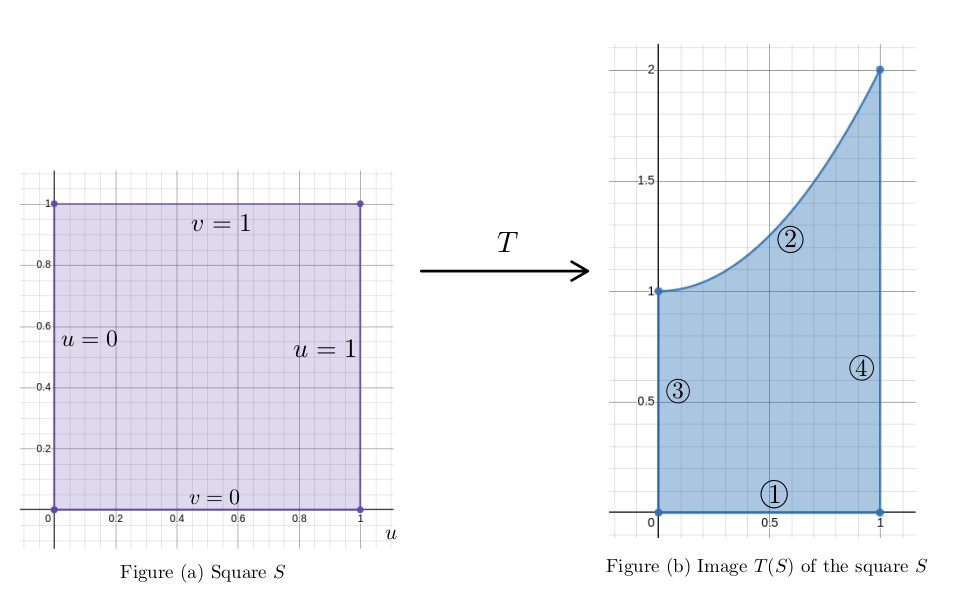
\includegraphics[scale=0.5]{prob8-15-9.png}
	\end{center}
	It's like if $S$ was stretched from one of its corners. \hfill $\triangle$
\end{document}